\documentclass[titlepage, a4paper, 11pt]{scrartcl}

%too much whitespace otherwise
\usepackage[left=2cm,right=2cm,top=2cm,bottom=2cm]{geometry}

% Grafik Pakete
\usepackage{graphicx,hyperref,amssymb}

% Ordner für Grafiken
\graphicspath{ {./images/} }
\usepackage{float}

\usepackage[utf8]{inputenc}
\usepackage{amsmath}
\usepackage{amsfonts}
\usepackage{amssymb}
\usepackage{graphicx}

\usepackage{caption}
\usepackage{subcaption}

% Header and Footer
\usepackage{fancyhdr}

%bibtex
\usepackage{cite}

%code snippets
\usepackage{listings}
\usepackage{color}

\definecolor{dkgreen}{rgb}{0,0.6,0}
\definecolor{gray}{rgb}{0.5,0.5,0.5}
\definecolor{mauve}{rgb}{0.58,0,0.82}

\lstset{frame=tb,
    language=HTML,
    aboveskip=3mm,
    belowskip=3mm,
    showstringspaces=false,
    columns=flexible,
    basicstyle={\small\ttfamily},
    numbers=none,
    numberstyle=\tiny\color{gray},
    keywordstyle=\color{blue},
    commentstyle=\color{dkgreen},
    stringstyle=\color{mauve},
    breaklines=true,
    breakatwhitespace=true,
    tabsize=3
}

\pagestyle{fancy}
\fancyhf{}
\rhead{Julius Neudecker, 2025850}
\lhead{CEPH Cluster in containers}

\title{Running a CEPH-Cluster from a containerized infrastructure}
\subtitle{Use case: mySQL-database}
\author{Julius Neudecker \\ Bachelor of Science \\ \href{mailto:julius.neudecker@haw-hamburg.de}{julius.neudecker@haw-hamburg.de}}
\date{January 2020}


\begin{document}

    \maketitle

    \tableofcontents

    \begin{abstract}
        %Setting up and operating a storage cluster with high availability is a complex task. 
        %Modern paradigms like containerization and orchestration are a way of abstracting away some these complexities.
        %However, running a fault resistant storage cluster in a stateless and ephemeral containerized environment might seem contradicting at first.
        %Therefore the following paper will adress these problems, scrutinize performance and point out the inherent keypoints of this concept.
        %To put this analysis into context, a mySQL database will act as a use case to create a frame of reference.

        %An abstract summarizes, usually in one paragraph of 300 words or less, the major aspects of the entire paper in a prescribed sequence that includes: 
        %1) the overall purpose of the study and the research problem(s) you investigated; 
        %2) the basic design of the study; 
        %3) major findings or trends found as a result of your analysis; and, 
        %4) a brief summary of your interpretations and conclusions.

        Setting up and operating a storage cluster with high availability is a complex task. 
        By using containerization, it is possible to abstract away and encapsulate some repetitive tasks.
        Therefore this study aims to analyse the possibility, implications and findings of a multi host
        CEPH-Cluster, where the individual daemons are entirely running within a containerized environment.
        To put the findings into a frame of reference, this study utilizes a mySQL-database which has 
        special requirements on data storage. The key points in terms of advantages and disadvantages,
        data integrity, performance and administion are scrutinized. Major findings are that ...
        [insert findings here later] ... .
        Therefore running a distributed CEPH-storage in a containerization environment is ... 
        [draw conclusion] ... .



    \end{abstract}

    \section{Introduction}

        In times where information is a valuable asset, it is of paramount importance to have a scalable and reliable
        way of storing data and information. Considerations about data throughput and 
        IOPS\footnote{Input/Output Operations per Second} are also a major design parameter on modern storage solutions.
        These different storage solutions provide different approaches on these considerations. For any given use case, there
        exist several options to adress these. Depending on the architecture and scope of the problem some are better
        suited than others. A few major considerations are apart from scalability, reliability and speed also cost effectiveness,
        vendor lock-in, complexity and granular customizability.

        In general hardware based solutions have advantages in terms of raw performance but they often have significant disadvantages
        when it comes to vendor lock-in, easy scalability or restoration of corrupted disks. Software and network based solutions are
        \textit{in principle} less performant. However this can be mitigated for the most part by scaling up.

        Apart from propretary cloud storage providers i.e. AWS, Azure or Google, the \textbf{free market [correct term?]}
        is heavily dominated by CEPH by more than twice as much as the next competitor:

        \begin{figure}[H]
            \centering
            \fbox{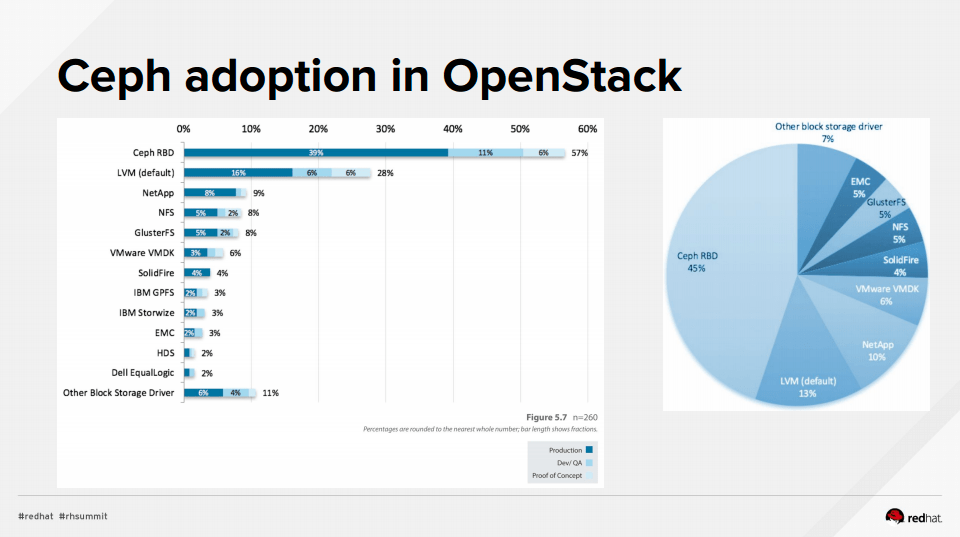
\includegraphics[width=0.95\textwidth]{marketshareCeph.png}}
            \caption{Adoption of CEPH in OpenStack in 2016, \cite{ceph}}
            \label{fig:ceph-market-share}
        \end{figure}

        Being conceived by Sage Weil for his doctoral thesis\cite{weil2007ceph}, CEPH became part of the Linux Kernel in 2010 and was acquired
        by RedHat in 2014, CEPH is gaining popularity steadily since its introduction. \textbf{Source?}

        \bigskip

        Another modern important concept which is increasingly shaping modern technology stacks is \textit{OS Level Virtualization} or
        \textit{containerization} as its colloquially called. This way of deploying applications decreased the complexity, which is
        inherent to deploying several different applications to one single host machine. \textbf{[Since when?]}
        One integral property of these \textit{containers} is that they are stateless and ephemeral. This means that they can 
        \textit{by principle} be created and deleted according to momentary requirements. 

        \bigskip

        In this paper both technologies will be utilized to overcome some properties of these two technologies by merging them 
        and thus using synergies \textbf{[really?]}


        \subsection{Scope of the problem}
        %Managing a highly available storage cluster is not a trivial task. Apart from provisioning and monitoring the hardware,
        %setting up multiple systems concurrently is a daunting task. Nowadays with provisioning tools like Salt, Chef or Puppet, 
        %this is easier than ever. However

        %Docker, stateless, ephemeral vs database, acid,

        %do some sidestep to open stack and the RedHat Paper and why ceph blabla

        %do some explanation about single/multi tennant and cloud
 
        %put the whole paper in the context of IAAS; PAAS; SAAS

        % make a remark on which particular issue this paper adresses, since there are way too many 
        % to discuss and thats beyond this paper.

        \subsection{CEPH Based storage cluster}

        % librados, radosgw, rbd, cephfs (build on top of krbd/librados -> source?)
        % quick rundown of MON, OSD, MDS, MGR

        \subsection{Containerization}

        %whats a container and why is it nice compared to VM, etc.

        \subsection{Databases}

        % quick rundown. Focussed on mySQl, mention of noSQL, etc.

        \subsection{Definition of research goal}        

        % with/without container

        \subsection{Related Work}
        %related work: redhat document

    \section{Setting up CEPH on Docker}

        \subsection{CEPH Architecture}
            
            \subsubsection{Monitor Nodes}

            % even/odd number and therefore need for odd number of servers

            \subsubsection{Object Storage Devices}

            % container config: different config options:
            % essentially: how much work is abstracted away from container

            \subsubsection{Metadata Service}

            \subsubsection{Manager}    

        \subsection{System Architecture}

        % three servers, one mon per machine
        % different number of OSD per machine
        % connected via docker network bridge

            \subsubsection{Orchestration with Kubernetes (or Docker Swarm maybe...)}

            \subsubsection{CRUSH Fail mode}

            % elaborate different settings: Datacenter, Room, Row, Rack, Host, OSD...
            % this has to be taken into consideration for providing the data on a global scale

            % host vs osd in this case

            % assuming all disks are _equally_ new, host mode would be appropriate in this setting
            % in this particular case I would choose OSD level since disks are of different type, age and degradation

            \subsubsection{Issue with Docker Image}

            % refer to https://hub.docker.com/r/ceph/daemon 
            % workaroung with either multiple OSD per container (undesireable)
            % or different thing -> What are the implications anyway?


        
    \section{Database considerations}

        \subsection{Architecture of mySQL}

        % why onfirst sight it might not be ideal to deploy mySQL on ceph because of distributed nature
        % and in case of Table > volume, etc.
        % architecture: https://www.youtube.com/watch?v=CCqFqraSQQ0

        \subsection{ACID}

        % Atomic, Consistent, Isolated, Durable
        % https://www.youtube.com/watch?v=VRm2UMsFVz0

        % whats acid and why is it important in this context
        % is it actually an issue?!

        % i.e. concurrent transactions
        % example: bank account

        \subsection{Problems with clusters}

        %sharding and distribution techniques
        %splitting up of big files over OSD

        \subsection{Considerations for this research}

    \section{System Analysis}

        % what are the key points to analyze in the context

        \subsection{Disclaimer}

        [Bc of Corona I can't use lab therefore only my setup. Discuss some shortcomings and implications.]

        % my setup is a multi tennant system, so take everything with a grain of salt.
        % however: disks were single tennant

        %cannot setup "native" environment, make reasonable assumptions based on other research

        \subsection{Data Integrity}

        %distribution over PG, OSD, Hosts

        %CEPH data striping:
        % https://access.redhat.com/documentation/en-us/red_hat_ceph_storage/1.2.3/html/red_hat_ceph_architecture/ceph_client_architecture#:~:text=Object%20Size%3A%20Objects%20in%20the,%2C%204MB%2C%20etc.).

        \subsection{Performance Penalty}

        %CephFS vs. Librados vs. native

        % IOPS vs raw throughput
        % the point is: does docker make a difference here?

        \subsection{Administration}

        % Ceph Dashboard
        % Grafana mySQL          


        \subsection{Tuning}

        [very briefly]

        % KVM vs QEMU
        % librbd vs krbd
        % percona container in krbd module vs. mysql docker on librbd
        % other tuning parametres

    \section{Conclusion}

        \subsection{Advantages}

        %in comparison to conventional (Host Level)

        \subsection{Disadvantages}

        %in comparison to conventional (Host Level)        

        \subsection{Performance}
    
        % make remark about performance tuning and tiering -> beyond the scope of this
        % i.e. pool configs, stripe config, safety with crush config, etc.
        % also there might be another interface for mySQL needs like RADOSGW or RBD
        % but this would not be comparable to a single tennant mySQL application

        %which implementation of radoes does the container use? krbd vs librbd
        % remark to section with OSD in Architecture: "ease of use" vs "performance" tradeoff

        \subsection{In Summary}

        % summarize the keypoints in regard to the introduction
      

    \bibliography{literature}        
    \bibliographystyle{IEEEtran}

\end{document}